\documentclass[10pt, conference, compsocconf]{IEEEtran}

\ifCLASSINFOpdf
 \usepackage[pdftex]{graphicx}
 \graphicspath{{SupportFiles}}
 \DeclareGraphicsExtensions{.pdf,.jpeg,.png}
\else
\fi
\usepackage[cmex10]{amsmath}

\begin{document}
\title{A Survey on Automated Software Repair}

\author{\IEEEauthorblockN{Rifatul Islam}
\IEEEauthorblockA{Graduate Teaching Assistant\\
Department of Computer Science\\
University of Texas at San Antonio\\
rifatul.islam@utsa.edu}


}

\maketitle
\thispagestyle{plain}
\pagestyle{plain}

\begin{abstract}
This paper presents an insightful analysis of some of the state-of-the-arts in the field of frequent pattern mining over uncertain databases. The two directions of the uncertainty model have been studied deeply. Three well known algorithms U-Apriori, UH-mine and PUF-Growth have been analyzed in the expected support based framework. Another framework is probabilistic support in which computation is the main challenge. More three algorithms PFPM(Probabilistic Frequent Itemset Mining), DC(Divide and Conquer based Mining) and ProFp-Growth are presented along with their different probabilistic support computation scheme. In comparative analysis, the computational cost, memory requirement along with the architectural overview of the algorithms have been presented. The performance of the mentioned algorithms is studied with different uncertain database parameters. Finally, some future research directions are identified to proceed in this area. This survey on the uncertain frequent pattern mining enable a novice researcher to understand the basic uncertainty model and design methodology of the existing algorithms.


\end{abstract}

\begin{IEEEkeywords}
Uncertain Data Mining, Frequent Pattern Mining

\end{IEEEkeywords}


% For peer review papers, you can put extra information on the cover
% page as needed:
% \ifCLASSOPTIONpeerreview
% \begin{center} \bfseries EDICS Category: 3-BBND \end{center}
% \fi
%
% For peerreview papers, this IEEEtran command inserts a page break and
% creates the second title. It will be ignored for other modes.
\IEEEpeerreviewmaketitle


%======================================================
\section{Introduction}
Today the world is inundated with massive amount of data. Very valuable implicit information are hidden within  these data which can be used to make decision support system more effective. Frequent pattern mining is one of the basic task of data mining that is used in the association rule mining to facilitate the decision making efficient.
Frequent pattern mining aims to discover  previously unknown and potentially useful knowledge - revealing patterns on collection of frequently co-occurring items or events - that are embedded in data.



At the beginning, the frequent pattern mining algorithms were based on databases where the items or events were certainly present in a transaction within the database. Like in Table-\ref{table:certain}, items are either present or absent in a transaction as indicated by their value as $0$ or $1$. The frequent pattern mining algorithm aims to discover patterns or itemsets those having a certain minimum user specified support threshold (i.e., the database coverage) in the database. Like if you want to mine patterns that would have $50\%$ support or coverage in the database in Table-\ref{table:certain}, then the patterns $\big\{ b \big\}$, $\big\{ c \big\}$, $\big\{ b, c \big\}$ will be revealed because these patterns have appeared in both the transactions and their support or frequency is $66.67\%$. If the Table-\ref{table:certain} database is a transactional database of a shop, then from the pattern $\big\{ b, c \big\}$ the owner can decide to put item $b$ alongside $c$ for raising sell as the both items are frequently bought by most of the customers.

In recent years the availability of uncertain data has raised due to the result of new methodologies of data collection. With many applications such as sensor network monitoring, moving object search, protein-protein interaction network analysis are producing data whose nature is uncertain. Uncertainty can be caused by (i) our limited perception or understanding of reality; (ii) limitations of the observation equipment; or (iii) limitations of available resources for the collection, storage, transformation, or analysis of data. It can also be inherent in nature (say, due to bias). Data collected by chemical, electromagnetic, thermal sensors in environment surveillance, security, and manufacturing systems can be noisy. Dynamic  errors - such as (i) inherited measurement inaccuracies, (ii) sampling frequency of the sensors, (iii) deviation caused by a rapid change (e.g., drift, noise) of the measured property over time, (iv) wireless transmission errors, or (v) network latencies - also introduce uncertainty into the data reported by these sensors. As an example of uncertain database consider the Table-\ref{table:uncertain}. Here each row indicates a customer and reflects their probability or likelihood of buying an item. Where each customer row is produced by aggregating the information from the transactional history of that particular customer.


\begin{table}
\parbox{.45\linewidth}{
\centering
\begin{tabular}{| c | c | c | c|}\hline
TID & a & b & c\\ \hline  \hline
$t_1$ & 1  & 0 & 0 \\ \hline
$t_2$ & 0  & 1 & 1 \\ \hline
$t_3$ & 0  & 1 & 1 \\ \hline
\end{tabular}
\caption{Certain Database}
\label{table:certain}
}
\hfill
\parbox{.45\linewidth}{
\centering
\begin{tabular}{| c | c |}\hline
TID & Items \\ \hline  \hline
$t_1$ & (a,0.2),(b,0.9),(c,0.4) \\ \hline
$t_2$ & (a,0.6),(b,0.6),(c,0.6),(d,0.9) \\ \hline
$t_3$ & (a,0.6),(b,0.5),(d,0.5),(e,0.7) \\ \hline
$t_3$ & (a,0.9),(b,0.2),(c,0.8),(e,0.3) \\ \hline
\end{tabular}
\caption{Uncertain Database}
\label{table:uncertain}
}
\end{table}

Now, uncertainty in the database poses new challenges to the researchers - how to extract implicit information from the database. The frequent pattern mining algorithms so far developed become obsolete due to that frequency or support of a pattern can not be calculated same as the certain database. New semantic analysis is required to define frequency of a pattern in uncertain environment. Researchers have come up with an idea of Possible World Semantics that is commonly used in frequent pattern mining. When an item $x$ is in a transaction then there can exist two possible worlds such that (i) a possible world where $x$ is present in $t_i$ (i.e., $x$ $\in$ $t_i$) (ii) another possible world where $x$ is not present in $t_i$ (i.e., $x$ $\notin$ $t_i$). If there are $|DB|$ number of transactions in the database and $|I|$ number of distinct items in the database, then $2^{|DB|.|I|}$ number of possible worlds can exist. Based on this semantic, there are two ways to define the probabilistic frequency as (i) expected support, (ii) probabilistic support. Different algorithms have been proposed in the literature based on this two distinct support metrics. The required terms and definitions will be provided in their corresponding sections.



\section{Expected Support Based Algorithms}
In this section, we will discuss the basics of expected support and corresponding three representative algorithms. Expected support based algorithms use expected support which is a measure of uncertainty and simply an adaptation of support or frequency of a pattern in certain database. In the following section, some basic terms and definitions will be discussed which will facilitate better perception on the expected support based uncertain framework.

Let $DB = \{t_1, t_2, t_3, \ldots ,t_n\}$ be the uncertain database, $I = \{i_1, i_2, i_3,  \ldots ,i_m\}$ be the set of distinct items in the itemset. For brevity, lets denote a pattern or itemset as $X = \{x_1, x_2, x_3, \ldots ,x_k\}$. Pattern $X$ is called $(k-itemset)$ if it contains $k$ distinct items. A  transaction $t_i$ denoted as $TID = \{ (x_1, p_1), (x_2, p_2), (x_3, p_3), \ldots ,(x_k,p_k)\}$ such that each item $x_i$ has an existential probability $p_i$ (i.e., likelihood of an item appeared in $TID$) associated with it. Given the details, the expected support of a pattern is defined as the following equation,

\[
 expSup(X, DB) = \sum_{i=1}^{|DB|} ( \prod_{x \in X} P(x, t_i)) 
\]

Formally, the expected support of a pattern $X$ in uncertain $DB$ can be computed as a sum (over all $DB$ transactions) of the product of existential probabilities of all items within $X$. Given (i) an uncertain database $DB$, (ii) a user specified minimum expected support threshold $min\_esup$, then the problem of mining frequent pattern can be defined as finding all of the patterns $X$ having $expSup(X) \geq min\_esup$ from the database. Such a pattern $X$ is called expected support based frequent pattern or frequent pattern for short. In the subsequent subsections, three expected support based algorithms will be briefly described.

\subsection{U-Apriori Algorithm}
U-Apriori \cite{Chui2007} is the first algorithm which is a level-wise breadth first search strategy based on candidate generation and testing framework. U-Apriori first computes the expected support of all the distinct items from the itemset of the database. Then it compares their expected support with respect to $min\_esup$, and it generates a set of $(itemset-1)$ (which contains all the single items whose expected support is greater than or equal to $min\_esup$). After that U-Apriori joins $(itemset-1)$ with $(itemset-1)$ to generate the candidate set of $(itemset-2)$ and check each of the itemset from $(itemset-2)$ with respect to $min\_esup$ and finally it removes the itemsets from $(itemset-2)$ whose expected support is less than $min\_esup$. In this way, U-Apriori repeatedly generates $(k+1-itemset)$ from $(k-itemset)$ and test the itemsets from the candidate set. This process ends when there is no candidate set generated. U-Apriori also relies on Apriori property (also known as downward closure property or anti-monotonic property) from the Apriori algorithm designed for certain database. Apriori property is defined as if an itemset is frequent then all of it's subsets must be frequent. Subsequently, all supersets of an infrequent pattern must also be infrequent. This traditional Apriori pruning also applies in U-Apriori. When generating $(k+1-itemsets)$ from $(k-itemsets)$, an itemset is included in $(k+1-itemsets)$ if and only if it's all subsets are in $(k-itemsets)$.

In addition to the previously explained pruning scheme, another scheme as decremental pruning is also proposed for further improving the mining execution time. This technique basically tries to determine the upper bound of an itemset or pattern as early as possible. If the upper bound falls lower than the $min\_esup$, then the itemset is immediately discarded from the candidate set.

\subsection{PUF-Growth Algorithm}
In this subsection, another expected support based frequent mining algorithm PUF-Growth \cite{Leung2013} will be described briefly which is a tree based depth first search approach to mine uncertain frequent patterns. It is an adaptation of classic Fp-Growth algorithm for mining frequent patterns from certain database. This work does an improvement on a sequential development of tree based mining approaches. It generally builds a tree to capture the whole database. Initially, a single transaction is sorted according to the item's appearance frequency (i.e., highest frequent item will be in front of the list), then the sorted list is inserted into the tree. In this process, the frequent items will be close to the root and will share a common prefix among the transaction which resulted into a more compact tree. Then based on this tree, the mining algorithm will recursively builds conditional  projected trees and find frequent patterns from the projected trees.

\begin{figure}
\begin{center}
%\includegraphics[bb=2.0in 2.0in 3in 2in]{sfcompo.eps}
  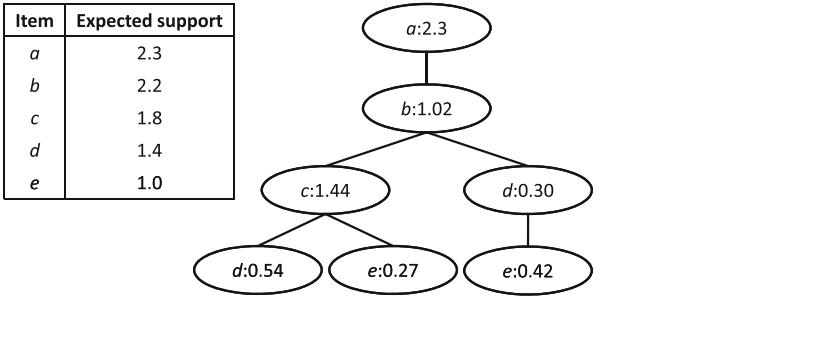
\includegraphics[height=5cm,width=\linewidth]{./Figures/puf.png}
\end{center}
  \caption{PUf-tree for the uncertain database in Table-\ref{table:uncertain}
  \label{puf}}
\end{figure}

In PUF-Growth algorithm, authors proposed an estimation of the expected support of a pattern or itemset which is defined as prefixed item cap, which will tighten the upper bound more. The prefixed item cap - denoted as $I^{Cap}(x_r,t_i)$ of an item $x_r$ in transaction $t_i = \{ x_1, \ldots ,x_r, \ldots ,x_h\}$, where $1\leq r \leq h$ (i.e., $h=|t_i|$ represent the length of $t_i$), is defined as the product of $P(x_r,t_i)$ and the highest existential probability value M of the items from $x_1$ to $x_{(r-1)}$ in $t_i$. More  formally,



\[
    PIcap(x_r,t_i)=\left\{
                \begin{array}{ll}
                    P(x_r,t_i) * M; \quad \textrm{if} \quad |t_i| > 1\\
                  P(x_1,t_i); \quad \textrm{if}  \quad |t_i|=1\\
                  
                \end{array}
              \right.
  \]

where $M$ = $max_{q \in [1, r-1]} P(x_q,t_i)$.



In the first scan of the database, PUF-growth computes the prefixed item caps. In the second database scan, the  PUF-tree is built where each node contains an item identifier and the corresponding prefixed item cap. There is also a header table which contains a cell in a list for each distinct items in the PUF-tree. The cell consists of three elements (i) item identifier, (ii) expected support and (iii) link to a same item node in the PUF-tree. PUF-growth algorithm then projects the PUF-tree into more smaller projected trees recursively based on the each items in the header table and mines frequent patterns from those smaller projected trees.

The frequentness of the patterns is based on the upper bound of the probable expected support not the actual expected support. Thus after completion, the PUF-growth algorithm mines patterns which includes false positive patterns. A third database scan is needed to calculated the actual expected support  of the patterns as  well as to discard the false positives. The number of false positives are much less than the previous tree based algorithm for the tight bound of prefixed item cap. 

\subsection{UH-mine Algorithm}
\begin{figure}
\begin{center}
%\includegraphics[bb=2.0in 2.0in 3in 2in]{sfcompo.eps}
  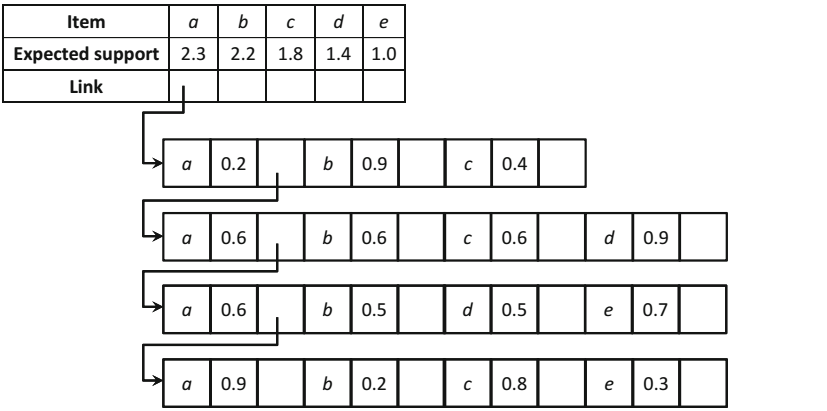
\includegraphics[height=5cm,width=\linewidth]{./Figures/uh.png}
\end{center}
  \caption{UH-structs for the uncertain database in Table-\ref{table:uncertain}
  \label{uh}}
\end{figure}

In this subsection, we will discuss another divide and conquer and depth first search strategy based method named UH-mine \cite{uhmine}. This algorithm is extended from classical H-mine algorithm for mining frequent patterns from certain database. UH-mine can be explained as follows. The UH-mine algorithm adopts a hyperlinked data structure called UH-struct which contains (i) the label of the item, (ii) the corresponding existential probability of the item and (iii) the hyperlink to point to the item to the next UH-struct. Initially, UH-mine scans the input database once to find the frequent items. The infrequent items are removed from the database. The frequent items left in each input transaction are sorted according to a certain global ordering scheme. Then for each transaction in the database the UH-structs are built. Then the head table is built with the frequent items which were passed from the first database scan. The head table contains (i) label of the item, (ii) the corresponding expected support of that item and (iii) the hyperlink to the first UH-struct that contains the item. From the Figure-\ref{uh}, it can be seen from the head table, the expected support of the item $a$  is 2.3 and the hyperlinks that connects $a$ in the first UH-struct. After the global UH-struct construction, each item in different UH-structs are connected by the hyperlinks and from the head table it can be traversed through all of the UH-structs those contain that particular item.

During the mining process, a prefix itemset exists (lets denote it as $X$ and which is initially empty). UH-mine uses the head table which records the starting points of the projected database. By following the links in the head table, UH-mine can locate all the projected transactions and find the locally frequent items by scanning the projected database. The locally frequent items w.r.t the prefix $X$ can be used to extend $X$ to longer prefix itemsets. There are two ways to mine uncertain frequent patterns with the prefix $X$. The first approach is to maintain the probability $P(X, t_i)$ of prefix $X$ occurring in each projected transaction $t_i$ in memory. As the probability of the presence of locally frequent item $x$ in transaction $t_i$ is recorded in the UH-struct, it is easy to compute the expected support of the new itemset $\{X \cup x\}$ as $P(X, t_i) * P(x, t_i)$. In addition to that, the expected support of prefix $X$ with respect to each conditional database needs to be maintained until all the locally frequent items w.r.t. prefix $X$ have been processed. The other approach is to avoid maintaining the the probability of prefix $X$. As the UH-struct contains the existential probabilities of all the item's in the prefix $X$, then it is easy to compute new extended itemset $\{X \cup x\}$ as $P(X, t_i) * P(x, t_i)$ on the fly.








\section{Exact Probabilistic Frequent Pattern Mining}
In this section, we will discuss some of the basics needed to understand the exact probabilistic support of an itemset or pattern. Then we will define the probabilistic frequent pattern mining problem. In the following subsections, three representative algorithms (i) PFPM (Probabilistic Frequent Pattern Mining), (ii) DC (Divide and Conquer based Apriori Algorithm) and ProFp-Growth will be presented briefly.

 According to the probabilistic frequent itemset, the probability that an itemset appears at least the minimum support ($min\_sup$) times is defined as the measurement, called as the frequent probability of an itemset, and an itemset is frequent if and only if the frequent probability of such itemset is larger than a given probabilistic threshold.

The Possible World Semantic is the basis for the computation of probabilistic frequent pattern. The probability that a  possible world exists is computed as follows:

\[
P(w) = \prod_{t \in I} (( \prod_{x \in t_i} P(x \in t_i)) * \prod_{x \notin t_i} ( 1 - P(x \in t_i)))
\]

where I is set of all distinct items in the database and $t_i$ is the transaction in the database.

In uncertain transaction databases, the support of an item or itemset cannot be represented as a unique value, it must be represented by a discrete probability distribution according to support. Now given an uncertain transactional database $DB$ and  $W$ be the set of all the possible worlds based on $DB$, the support probability of an itemset $X$ as $P_i(X)$ for specific support $i$ can be calculated as follows:

\[
P_i(X) = \sum_{w_j \in W, (sup(X, w_j)=i)} P(w_j)
\]
where $sup(X,w_j)$ is the support of $X$ in the world $w_j$.

Now given a user specified minimum support threshold $min\_sup$, the frequentness probability of an itemset $X$ is defined as follows:
\[
P_{\geq min\_sup} (X) = \sum_{i=0}^{min\_sup} P_i(X)
\] 

Given (i) uncertain database, (ii) minimum user support threshold $min\_sup$ and (iii) probabilistic frequent threshold $pft$, then the problem of mining uncertain frequent patterns is to find all the patterns $X$ having $P_{\geq min\_sup} \geq pft$.

\subsection{PFPM Algorithm}
As the probabilistic support computation involves huge number of possible world's probability calculation for all of the support value $\{0,1,2, \ldots min\_sup\}$, so it requires an efficient computation. In PFPM \cite{pfpm}, the authors have proposed a dynamic programming based algorithm to compute the support probability. For simplifying the following discussion, lets define that $Pr_{\geq i,j}(X)$  denotes the probability that itemset $X$ appears at least $i$ times in the first $j$  transactions in the given uncertain database. $Pr(X \subseteq t_j)$ is the probability that itemset $X$ appears in the $j$ th transaction $t_j$. $|DB|$ is the number of transaction in the database. The recursive relation for the dynamic programming can be defined as follows:

\[
\begin{aligned}
Pr_{\geq i,j}(X)=Pr_{\geq i,j}(X)*Pr(X \subseteq t_j) \\
+ Pr_{\geq i,j-1}(X)*(1-Pr(X \subseteq t_j))
\end{aligned}
\]

\[
\textrm{Boundary case}=\left\{
                \begin{array}{ll}
                    Pr_{\geq 0,j}(X) = 1; \quad 0 \leq j \leq |DB|\\
                  Pr_{\geq i,j}(X) = 0; \quad i > j\\
                \end{array}
              \right.
\]

Thus, the frequent probability computation is $Pr_{\geq min\_sup,|DB|}(X)$. PFPM adopts the Apriori approach for mining the frequent patterns. 

\subsection{Divide and Conquer based Algorithm}
Another approach DC \cite{todis} has been proposed for calculating probabilistic frequent patterns based on divide and conquer methodology besides the dynamic programming approach. In this computation  method, the uncertain database $DB$ is partitioned into two equal small partitions as $DB_1$ and $DB_2$. Then, in the two smaller databases, the  algorithm recursively calls itself to divide the database until a single transaction left. Then the algorithm computes the probabilistic frequentness of the itemset in that transaction. Finally, conquering the results the final probabilistic frequentness is calculated when the program terminates. To speed up the computation, DC method uses Fast Fourier Transformation  in the conquering part. Rather than computing the probabilistic frequentness in a different manner, DC approach also enumerates frequent patterns following the Apriori approach same as the PFPM.

\subsection{ProFp-Growth Algorithm}
In this subsection, we will present another tree based probabilistic frequent pattern mining algorithm ProFp-Growth \cite{profp}. As the name implies, it's an adaptation of FP-growth algorithm. In this paper, authors have come up with a new probabilistic support computation scheme which is based on generating function. This algorithm also requires a tree (i.e., ProFp-tree) to capture the uncertain database. ProFp-tree in this algorithm can be described by the three elements as follows:

(i) Uncertain item prefix tree : A $null$ rooted tree consisted of each of the transactions from the database. A node in the tree contains five items as (i) $n$, identifier of the item, (ii)  $count$ denotes the certain occurrence of $path(n)$, where $path(n)$ be the set of items from $root$ to $n$, (iii) $uft$ is the set contains the transaction identifiers in which transaction $n$ is uncertain, (iv) $ufp$ is the set contains the transaction identifiers in which transaction $n$ is certain but an item from $path(n)$ is uncertain and (v) link to the next node in the tree same as $n$ if any node exists.

(ii) Item header table : This table maps all items to the first node in the uncertain item prefix tree.

(iii) Uncertain item lookup table : This table maps each item with the existential probability for every transactions.

The ProFp-Growth mining algorithm runs almost the same manner as Fp-Growth. In the projected tree construction, the algorithm extracts the path to the $root$ and updates all of the parameters $count, uft$ and $ufp$ of each of the nodes in the path. It is slightly time consuming in comparison with the Fp-Growth algorithm. For the calculation of the probabilistic support, the corresponding existential probabilities are accumulated into a list of uncertain values by using the $uft$ list and from the uncertain item lookup table.

\section{Comparative Analysis}
In this section, we will present our observations regarding  the explained algorithms in the previous section. The analysis will include the runtime comparison, memory usage comparison as well as the algorithm's architectural evaluations. One of the basic criteria in evaluating the algorithm performance is based on the density of the database, which is defined as following:
 
 \[ \textrm{density} = \frac{\textrm{number of distinct items in the database}}{\textrm{number of transaction in the database}}\]
 
In the expected support based algorithms, the actual support or coverage of the database is ignored completely, it only relies on the expected support of an itemset. In this approach, the user has to provide a minimum expected support threshold which is also difficult to choose because of the density of the database and the probabilistic distribution of the database. It requires a trial and error method to pick a good expected support threshold, which can be problematic in some aspect.

U-Apriori algorithm needs $k$ number of database scans to mine $k-itemsets$ and the PUF-Growth algorithm needs three database scans whereas UH-mine algorithm requires database scan twice. An algorithm which requires more database scanning eventually requires more execution time. In dense database along with high minimum support, $min\_esup$, U-Apriori outperforms UH-mine because the computation is done on relatively small search space. In this scenario, breadth first search based algorithms perform well eventually. But, in sparse databases, UH-mine performs well with respect to U-Apriori. Although PUF-Growth is depth first search based algorithm but it requires to generate a number of projected trees on the basis of a prefix pattern recursively and it also involves en extra  database scan to filter out the false positives, so it can be slower in some specific database settings. From our observation, PUF-Growth might perform really well when the database is very dense and $min\_esup$ is very small,  then the resulted PUF-tree becomes very compact by sharing the common prefixes more frequently from the transactions in the database. Although, no comparison is found with the U-Apriori or UH-mine algorithm in the corresponding research papers.

In memory comparison scenario, U-Apriori is best obviously, because it does not depend on memory at all, it only requires to maintain the patterns list. UH-mine requires a only a snapshot of the in memory database and a head table. However,  PUF-tree is a compact database representation, it requires more memory for the recursive generation of the projected databases; so it is the most memory consuming algorithm. 

\begin{table}
\parbox{.90\linewidth}{
\centering
\begin{tabular}{| c | c |}\hline
Algorithm & Computation Cost\\ \hline  \hline
$PFPM$ & $|DB|^2.min\_sup$ \\ \hline
$DC$ & $|DB|.log(|DB|)$ \\ \hline
$ProFp-Growth$ & $|DB|.min\_sup$ \\ \hline
\end{tabular}
\caption{Probabilistic Support Computation Cost}
\label{comp}
}
\end{table}

In probabilistic frequent pattern mining algorithms, coverage or support of the database is also considered along with the existential probabilities of an itemset. Probabilistic support computation of an itemset requires the summation of the all possible worlds where that itemset exists. There are exponential number of possible worlds, trivially computing the probabilities of the possible worlds are practically infeasible. Thus how to compute probabilistic support of an itemset efficiently - becomes the main challenge in probabilistic frequent pattern mining. The probabilistic support computational cost of an itemset for the three algorithms are given in the Table-\ref{comp}. It is not hard to observe that the $DC$ requires the lowest computation cost. PFPM and DC both use the Apriori based candidate generate and test paradigm to mine frequent patterns, thus DC surely outperforms PFPM in any uncertain database as both have to test the same set of candidate patterns. ProFp-Growth also outperforms PFPM in any settings of the database. No runtime comparison is provided in  the corresponding papers between ProFp-growth and DC. However, we can observe that the computation cost for probabilistic support is less in DC. Now both algorithms have to generate the same number of frequent patterns. Also they both will test a lot of infrequent patterns. If the number of infrequent patterns tested in DC is less than the ProFp-Growth, then obviously DC will outperform ProFp-Growth. One of the main criteria to be considered to determine which algorithm is better is partially depends on the candidate patterns tested by the algorithms. Along with the candidate test overhead, there is also recursive tree generation cost is associated with the ProFp-Growth algorithm. An experimental evaluation is indeed needed to surface the actual result in different settings between these two algorithms.

\section{Conclusions and Future Works}
Now-a-days the number of uncertain databases are increasing rapidly. Thus, data mining task is required to surface the invaluable information embedded in the database. Frequent pattern mining is the most basic task to surface the hidden patterns which can be used to effective decision making. In this paper, we conduct a comprehensive study on some of the state-of-the-arts for uncertain frequent pattern mining. Since there are two definitions of frequent pattern in uncertain databases, most existing researches are categorized into two directions. From our study, it is clear that no single algorithm is best on different database settings (i.e., database density, item's probabilistic distribution, variation in $min\_esup$) for expected support based algorithms. The existing algorithms can be examined more deeply according to their various observed properties and new research can be conducted to devise new algorithm or hybridization of existing algorithms to overcome the previously mentioned problem. Accordingly, it can be further analysed to find out that if the  computation of probabilistic support of a pattern can be done in linear time.







 
%\input{02related}
%\input{03methodology}
%\input{04results}

%\section{Conclusions}
%\section*{Acknowledgment}
\IEEEtriggeratref{8}

\bibliographystyle{IEEEtran}
\bibliography{bib1}

\end{document}


